\subsection{Adimensionnement de l'équation~\ref{King-Pois}}
%	Pour adimensionner l'énergie, nous allons nous servir de la quantité $\sigma^2$. % qui à la dimension d'une énergie.
%	Nous introduisons la quantité $r_c$, pour adimensionner les distances, puis
%	nous faisons donc le changement de variable suivant :
	L'adimensionnement s'effectue avec $\sigma^2$ pour l'énergie et la longueur $r_c$ pour les distances. Ainsi :
	\begin{eqnarray*}
		\left\{\begin{array}{l}
			\gamma = \frac{\phi}{\sigma^2}\\
			x = \frac{r}{r_c}
		\end{array}\right.
	\end{eqnarray*}

	Il vient alors :
	\begin{equation}
		\frac{d}{dx}\(x^2\frac{d\gamma}{dx}\) = -\frac{4m\pi G r_c^2 \rho_0}{\sigma^2}x^2 \left\{-\sqrt{\frac{4\gamma}{\pi}}\(1 + \frac{ 2\gamma }{3}\) + e^{\gamma}\mathrm{erf}\(\sqrt{\gamma}\)\right\}
	\end{equation}

	Afin de compléter l'adimensionnement, nous prenons :
	\begin{equation}
		r_c^2 = \frac{\sigma^2}{4m\pi G\rho_0}
		\label{r_c}
	\end{equation}
	L'équation adimensionnée s'écrit alors :
	\begin{equation}
		\frac{d}{dx}\(x^2\frac{d\gamma}{dx}\) = x^2\frac{d^2\gamma}{dx^2} +
		2x\frac{d\gamma}{dx} = -x^2 \left\{-\sqrt{\frac{4\gamma}{\pi}}\(1 + \frac{ 2\gamma }{3}\) + e^{\gamma}\mathrm{erf}\(\sqrt{\gamma}\)\right\}
		\label{Pois-no_dim}
	\end{equation}

\subsection{Conditions aux limites}
	\subsubsection{Conditions au centre : $r=0$}
		\paragraph{Condition sur la dérivée :}
			Au centre de l'objet, toutes les forces ont des directions opposées --~le système étant isolé, son centre d'inertie est au repos~-- la
			somme des forces $\vec{F}=\sum_i\vec{f_i}$ est donc nulle. Ceci implique :
			\begin{equation}
				\sum_i\vec{f_i}(0)\cdot\vec{e_r} = m\frac{d\psi}{dr}(0) = 0
			\end{equation}
			Donc :
			\begin{equation}
				\left.\frac{d\gamma}{dr}\right|_{r=0} = \left.\frac{d}{dr}\(\frac{E_l - m\psi}{\sigma^2}\)\right|_{r=0} = -\frac{m}{\sigma^2}\left.\frac{d\psi}{dr}\right|_{r=0} = 0
			\end{equation}
		\paragraph{Condition sur la valeur du potentiel :}
%			L'énergie potentielle $m\psi(0)$ est l'énergie d'une particule du système n'ayant
%			pas de vitesse, il s'agit donc de l'énergie minimale d'une particule.
			En l'absence de vitesse, l'énergie minimale est atteinte pour la plus petit valeur de $m\psi(r)$, soit $m\psi(0)$.

			La quantité $\phi=E_l-m\psi$, où $E_l$ est l'énergie de libération,
			représente la quantité d'énergie à fournir à une particule à la distance $r$
			du centre du système pour qu'elle sorte du système. De plus, $\psi <0$, donc
			$\phi$ est positive ou nulle. Au centre, cette quantité vaudra :
			$$\phi(0)=E_l-m\psi(0)$$

			Nous prendrons donc la quantité initiale adimensionnée :
			\begin{equation}
				W_0 = \gamma(0)=\frac{E_l - m\psi(0)}{\sigma^2} > 0
				\label{W_0}
			\end{equation}

			Nous éviterons de la prendre nulle, car, dans ce cas, le système contient au
			plus une étoile.

	\subsubsection{Condition au bord : $r=R$}
		Au bord du système, les étoiles sont proches ou ont atteint la vitesse de
		libération, par conséquent nous avons :
		\begin{equation}
			\phi(X=R/r_c) = E_l - m\psi(X) \Rightarrow \gamma(X) = 0
		\end{equation}

		Le rayon $R$ de l'objet est donc fixé par le potentiel initial choisi.

\subsection{Paramètre du modèle}
	À ce point de l'étude, il devient évident que la physique du système va être dictée par le paramètre $W_0$ qui représente la quantité d'énergie qu'une particule va
	pouvoir gagner avant de ne plus être lié au système. Par conséquent, les paramètres $E_l$ et $\sigma^2$ vont être très importants : plus $\sigma^2$ (~la dispersion
	d'énergie~) est important, plus il va être facile de faire quitter le système à une partie des particules liées. Le raisonnement est similaire avec l'énergie de
	libération $E_l$ : plus cette énergie est proche de la valeur centrale du potentiel, plus le système va être petit, car l'énergie à récupérer pour sortir du système
	sera faible.

	Il n'existe que deux façons pour faire gagner de l'énergie à un particule en utilisant la gravitation : les collisions et le harcèlement de l'amas par un potentiel extérieur.
	Or le modèle de \textsc{King} doit être solution de l'équation de \textsc{Vlasov-Poisson}, il n'y a donc pas de collision. Un profil de \textsc{King} isolé ne doit donc pas évoluer.

	Dans la suite, nous considérerons donc le paramètre $W_0$ comme paramètre du système. Les quantités $E_l$ et $\sigma^2$ ne prendront toute leur importance que lorsque
	nous redimensionneront le problème.

\subsection{Adaptation à l'algorithme de résolution}
	L'algorithme que nous utiliserons pour résoudre cette équation est un \textsc{Runge-Kutta}
	d'ordre $4$ (~RK4~). Nous devons écrire l'équation différentielle comme un système d'ordre 1, ce que nous faisons en posant $u = \frac{d\gamma}{dx}$ :
	\begin{equation}
		\left\{\begin{array}{l}
			u = \x{\gamma}\\
			\\
			\x{u} = -\left\{-\sqrt{\frac{4\gamma}{\pi}}\(1 + \frac{ 2\gamma }{3}\) + e^{\gamma}\mathrm{erf}\(\sqrt{\gamma}\)\right\} - 2\frac{u}{x}
		\end{array}\right.
	\end{equation}

%	Euh .... Outre un problème évident de division par zéro en $x=0$, qui peut-être résolu à
%	l'aide d'un développement limité du potentiel au centre, lors de l'intégration, la solution
%	pour le potentiel est positive !!! \textcolor{red}{$\Rightarrow$ Normal, j'ai
%	oublié de repasser au potentiel !!! Je trace $\gamma$, et non $\psi$, qui est forcément
%	positif !!!}
	Un terme en $1/x$ est apparu, l'équation semble donc singulière en $0$. Un rapide
	développement limité de la fonction $\gamma$ autour de $0$ nous apprend qu'il n'en est rien, il n'y a
	pas de divergence. Pour éviter tout problème numérique, nous allons faire un développement limité d'ordre 6 autour de $0$.
	Les coefficients obtenu par ce développement sont :
%	Mais ce point va poser un problème numériquement. Nous allons donc
%	utiliser un  développement limité quand nous sommes autour de $0$. La calcul a été poussé à
%	l'ordre 6 sans preuve que les termes suivants soit négligeable. Le calcul des termes du
%	développement limité étant assez lourd à cause de la fonction $\mathrm{erf}$, il a été mené
%	avec l'aide de \textsc{Maple}. Voici les termes du développement ainsi obtenu :
	\begin{eqnarray}
		\left\{\begin{array}{l}
			\gamma(0) = W_0 \\
			\gamma'(0) = 0 \\
			\gamma''(0) = -\frac{\rho(W_0)}{3\rho_0} \\
			%\gamma''(0) = \frac{1}{3}\(-e^{W_0}erf(\sqrt{W_0})+2\sqrt{\frac{W_0}{\pi}}+\frac{4}{3}\sqrt{\frac{W_0}{\pi}}W_0\) = -\frac{\rho(0)}{3\rho_0} \\
			\gamma'''(0) = 0 \\
			%\gamma^{(4)}(0) = -\frac{6\gamma''(0)}{5}\left\{-\sqrt{\frac{W_0}{\pi}} -
			%\frac{\sqrt{W_0}}{2 W_0\sqrt{\pi}} + \frac{e^{W_0}\mathrm{erf}\(\sqrt{W_0}\)}{2}
			%+ \frac{1}{2\sqrt{\pi W_0}}\right\} = \frac{2\rho(0)}{5\rho_0}\left\{\sqrt{\frac{W_0}{\pi}} -
			%\frac{e^{W_0}\mathrm{erf}(\sqrt{W_0})}{2}\right\} \\
			\gamma^{(4)}(0) = \frac{2\rho(W_0)}{5\rho_0}\left\{\sqrt{\frac{W_0}{\pi}} -
			\frac{e^{W_0}\mathrm{erf}(\sqrt{W_0})}{2}\right\} \\
			\gamma^{(5)}(0) = 0
		\end{array}\right.
	\end{eqnarray}
	Nous avons alors les développements suivant autour de $0$ :
	\begin{align}
		\Rightarrow \gamma(x) &=& W_0 - \frac{\rho(W_0)}{3\rho_0}\frac{x^2}{2!} + \frac{2\rho(0)}{5\rho_0}\left\{\sqrt{\frac{W_0}{\pi}} -
		\frac{e^{W_0}\mathrm{erf}(\sqrt{W_0})}{2}\right\}\frac{x^4}{4!} + o(x^6) \notag \\
		\Rightarrow \frac{d\gamma(x)}{dx} &=& u = - \frac{\rho(W_0)}{3\rho_0}x + \frac{2\rho(0)}{5\rho_0}\left\{\sqrt{\frac{W_0}{\pi}} -
		\frac{e^{W_0}\mathrm{erf}(\sqrt{W_0})}{2}\right\}\frac{x^3}{3!} + o(x^5) \notag \\
		\Rightarrow \frac{d^2\gamma(x)}{dx^2} &=& \x{u} = \frac{\rho(W_0)}{3\rho_0} + \frac{2\rho(0)}{5\rho_0}\left\{\sqrt{\frac{W_0}{\pi}} -
		\frac{e^{W_0}\mathrm{erf}(\sqrt{W_0})}{2}\right\}\frac{x^2}{2!} + o(x^4) \notag
	\end{align}

	La résolution des équations nous permet alors d'avoir les graphiques de la
	figure~\ref{King_Modele-test} (~les graphes sont adimensionnés~).% mais pas normalisé~).
%	\paragraph{Problème : Résolu :}
%	Tant que la variable $x$ est proche de $0$, j'utilise les développements limités, puis passé
%	un certain seuil, je réutilise l'équation différentielle. Le résultat obtenu est la figure~\ref{King_Modele-err}
%	au lieu de la figure~\ref{King_Modele} (~figure pour laquelle je démarre à $x=1.10^{-6}$ au
%	lieu de $x=0$~). Il semblerait que mon algorithme de RK4 à pas variable ait du mal à suivre,
%	en plus d'avoir, apparemment, une erreur d'adimensionnement/normalisation.
%	\subparagraph{Solution pour le RK4 ne suivant pas :} J'utilisais le développement de $\gamma(x)$ pour calculer la pente
%	et celui de $\x{\gamma(x)}$ pour calculer la dérivée seconde.

%	\textcolor{red}{RAAAAAAHHHHHHHHH !!!!!!!!!! Plein d'erreur de signe dans les calculs et le
%	programme !!!!!!!!!!! Faut tout revérifier !!!!!!!!!!!!!!!!!!!}

%	\begin{figure}[ht!]
%			\begin{minipage}[b]{0.40\linewidth}
%				\centering 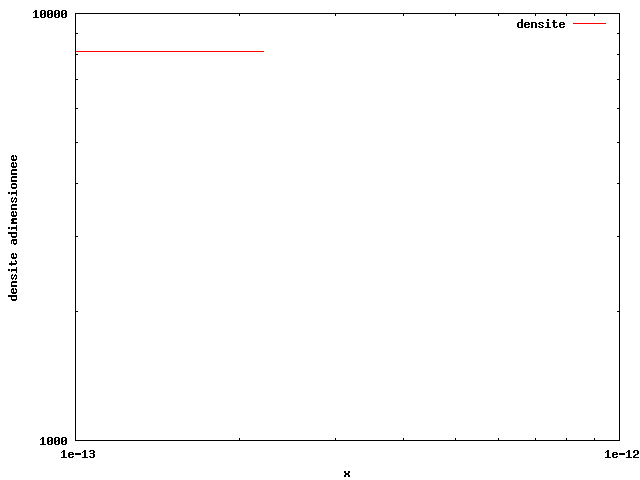
\includegraphics[scale=0.40]{graphe/erreur_king.png}
%			\end{minipage}\hfill
%			\begin{minipage}[b]{0.48\linewidth}
%				\centering 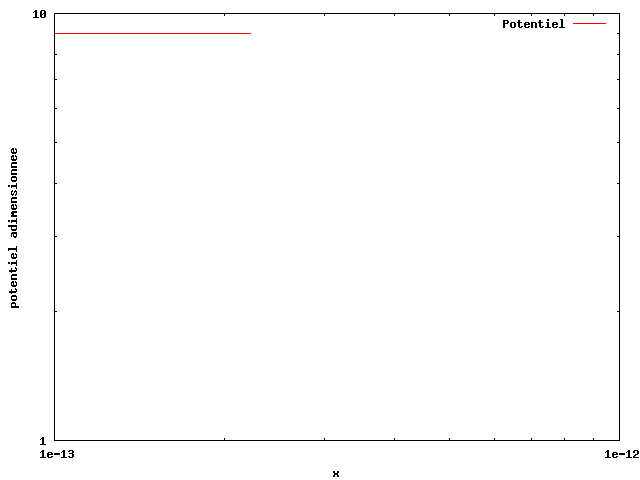
\includegraphics[scale=0.40]{graphe/erreur-pot_king.png}
%			\end{minipage}
%			\caption{Densité et potentiel d'un modèle de \textsc{King} pour les
%			conditions initiales (~au centre~) : $\gamma(0) = \frac{E_l -
%			m\psi(0)}{\sigma^2} = 9$}
%			\label{King_Modele-err}
%	\end{figure}
%	\begin{figure}[ht!]
%			\begin{minipage}[b]{0.40\linewidth}
%				\centering \includegraphics[scale=0.60]{graphe/densite_king.pdf}
%			\end{minipage}\hfill
%			\begin{minipage}[b]{0.48\linewidth}
%				\centering \includegraphics[scale=0.60]{graphe/potentiel_king.pdf}
%			\end{minipage}
%			\caption{Densité et potentiel d'un modèle de \textsc{King} pour les
%			conditions initiales (~au centre~) : $\gamma(0) = \frac{E_l - m\psi(0)}{\sigma^2} = 3$, $\x{\gamma}(0) = 0$}
%			\label{King_Modele}
%	\end{figure}

	\begin{figure}[ht!]
			\begin{minipage}[b]{0.40\linewidth}
				\centering \includegraphics[scale=0.60]{graphe/densite_pluri-king.pdf}
			\end{minipage}\hfill
			\begin{minipage}[b]{0.48\linewidth}
				\centering \includegraphics[scale=0.60]{graphe/densite_pluri_limite-king.pdf}
			\end{minipage}
			\caption{Densité d'un modèle de \textsc{King} pour les conditions initiales
			(~au centre~) : $\gamma(0) = 1$ (~courbe rouge~), $5$ (~courbe verte~), $9$ (~courbe bleu~), $14$ (~courbe violette~), $\x{\gamma}(0) = 0$}
			\label{King_Modele-test}
	\end{figure}

	La figure~\ref{King_Modele-test} montre l'aspect de la densité d'un modèle de \textsc{King} en fonction de $W_0$ et nous indique aussi que ce modèle posséde une structure cœur-halo
	(~une partie quasiment constante suivi d'une décroissance auto-similaire de pente $\alpha$~).
	Plus $\phi$ est grand, plus le cœur est dense (~le graphe de droite trace $\rho(x)/\rho(0)$~). Nous pouvons aussi observer que la pente n'est pas la même :
	elle diminue (~la courbe tend plus vite vers $0$~). Ce constat nous amène à nous poser une question : existe-t-il un
	lien entre la pente et le rayon du cœur ?
	\FloatBarrier
